The BitTorrent extension described in the previous section introduces a number of overheads. The introduction of an additional index at each node requires additional local storage space. Discovery of tracking data is achieved by having nodes make requests of relatively many other nodes. This requirement is likely to demand more bandwidth than the current BitTorrent protocol. We shall now quantify these overheads.

Bandwidth consumption is calculated using the following assumptions and generalisations about communication costs: 
\begin{enumerate}
    \item TCP/IP overhead amounts to 64 bytes per packet\footnote{\url{http://sd.wareonearth.com/~phil/net/overhead/}}
    \item We never send more bytes than can fit into a single packet (1500 bytes)
    \item BitTorrent requires an initial 51 bytes for a handshake\footnote{\url{http://bittorrent.org/beps/bep_0003.html}}
    \item BitTorrent adds 4 bytes of length prefix per message\footnotemark[\value{footnote}]
    \item A torrent infohash is 20 bytes\footnotemark[\value{footnote}]
    \item Results can be communicated using 6 bytes per node\footnote{Details of the IP and port for each node will make up the results list. \url{http://bittorrent.org/beps/bep_0023.html} explains how BitTorrent clients communicate IP:port combinations in 6 bytes.}
\end{enumerate}

\subsection{Single Node Sending Single Query}

    Using these assumptions we can estimate the communication cost for a node to send a query. For each query the node will contact $z$ other nodes, and receive a response from all of them. An unsuccessful response will contain no details of other nodes. A successful response will contain some number of results. A successful query is one in which at least one response was successful. For a successful query, the total cost depends on, (i) the number of successful requests and, (ii) the number of nodes listed in each response. For simplicity, we consider three cases; responses contain the details of a single node, of ten nodes and of 100 nodes. In practise, the size of a response will vary according to how many nodes each of the queried nodes are aware of. The cost, in bytes, to send a query is $z(64+51)=115z$. An unsuccessful response costs $64+4=68$ bytes. A successful response costs $64+4+6a=68+6a$ bytes, where $a$ is the number of results returned, $a=1,10,\textrm{ or }100$. The mean number of successful responses to a query can be determined by taking the expected value of the binomial distribution where each trial (each request) has probability of success $\displaystyle r(x)n^{-1}$. There are $z$ trials (requests) made per query and therefore $\displaystyle zr(x)n^{-1}$ successful responses on average. The expected cost of a query is:

    \begin{align}
        C_1 &= \textrm{cost to send query}\\
            &= 115z\\
        C_2 &= \textrm{cost to receive responses}\\
            &= 68z(1-r(x)n^{-1}) + (68 + 6a)zr(x)n^{-1}\\
          C &= \textrm{total cost for a single query}\\
            &= C_1 + C_2\\
            &= z(183 + 6ar(x)n^{-1})
    \end{align}

    Table~\ref{tab:single_query} shows cost of querying for torrents of varying popularity using several PAC Search strategies. Communication cost increases linearly with $z$ but we know from Eqn~(\ref{eq:prob_find_non_uniform_distribution}) that the probability of a successful query increases exponentially with $z$. When the tracking data is highly replicated, e.g. $x=10,000$, we observe that the communication cost can increase sharply with $a$. This is due to the fact that more of the $z$ queried nodes are able to respond with tracking data for such a high popularity torrent. Of course, for such a popular torrent, we can decrease $z$, and therefore the communication cost, and still maintain a high probability of success. For instance, if a torrent is owned by $x=10,000$ nodes then $r(x) >= 950,000$, substituting these values into Eqn~(\ref{eq:prob_find_non_uniform_distribution}) and using $P(d_i)=0.95$ we see that we would need only $z=15$. Such a query would cost less than 3KB, depending on the size of the responses. This example illustrates the need to adaptively adjust the size of the number of nodes queried, $z$, based on the awareness of a torrent. The difficulty is that a querying node is unlikely to know the awareness beforehand.  Given our assumption that a node repeats a query until successful, a simple strategy would be to initially query a small number of nodes and then to increase this value if a query is unsuccessful. A more detailed analysis of adaptively selecting the number of nodes queried is outside the scope of this paper, and we assume, for simplicity, that $z$ is fixed. The corresponding communication cost can therefore be considered a worst case estimate.

    \begin{table}
        \renewcommand{\arraystretch}{1.3}
        \caption{The communication cost, $C$, in bytes, for completing a single query for a torrent under different situations. The cost of the query is shown for different popularities, $x$, with varying numbers of nodes contacted, $z$, and also according to how many results are returned, $a$.}
        \label{tab:single_query}
        \centering
        \begin{tabular}{l|l|l|l|l|l|l}
            \hline
            \multicolumn{2}{c|}{Strategy} &   Popularity &     Awareness & \multicolumn{3}{|c}{Single Query Cost (bytes)} \\ \hline
                z &                   r(1) &            x &          r(x) &        $a=1$ &       $a=10$ &           $a=100$ \\ \hline
              100 &                  1,000 &            1 &         1,001 &        6,916 &            ~ &                 ~ \\
              500 &                  1,000 &            1 &         1,001 &       34,116 &            ~ &                 ~ \\
              500 &                  5,000 &            1 &         5,001 &       34,116 &            ~ &                 ~ \\
            1,000 &                  5,000 &            1 &         5,001 &       68,117 &            ~ &                 ~ \\ \hline
              100 &                  1,000 &           10 &        11,273 &        6,917 &        6,929 &                 ~ \\
              500 &                  1,000 &           10 &        12,986 &       34,122 &       34,183 &                 ~ \\
              500 &                  5,000 &           10 &        12,999 &       34,122 &       34,183 &                 ~ \\
            1,000 &                  5,000 &           10 &        15,843 &       68,129 &       68,251 &                 ~ \\ \hline
              100 &                  1,000 &          100 &        35,731 &        6,920 &        6,958 &             7,344 \\
              500 &                  1,000 &          100 &        60,505 &       34,137 &       34,330 &            36,259 \\
              500 &                  5,000 &          100 &        60,514 &       34,137 &       34,330 &            36,259 \\
            1,000 &                  5,000 &          100 &       105,080 &       68,158 &       68,544 &            72,403 \\ \hline
              100 &                  1,000 &        1,000 &       146,306 &        6,933 &        7,091 &             8,671 \\
              500 &                  1,000 &        1,000 &       486,543 &       34,203 &       34,993 &            42,894 \\
              500 &                  5,000 &        1,000 &       486,551 &       34,203 &       34,993 &            42,894 \\
            1,000 &                  5,000 &        1,000 &       912,316 &       68,291 &       69,871 &            85,672 \\ \hline
              100 &                  1,000 &       10,000 &       956,159 &        7,030 &        8,063 &            18,389 \\
              500 &                  1,000 &       10,000 &     3,170,983 &       34,689 &       39,852 &            91,485 \\
              500 &                  5,000 &       10,000 &     3,170,986 &       34,689 &       39,852 &            91,485 \\
            1,000 &                  5,000 &       10,000 &     4,328,606 &       69,263 &       79,589 &           182,854 \\
            \hline
        \end{tabular}
    \end{table}

\subsection{Authoring Node Bootstrapping}

    In order for a low popularity torrent to be discoverable in the network it is necessary for the few owning nodes to gossip details of themselves around the network. This is achieved by sending dummy requests to nodes. We have previously seen values of $r(1)=1000$ and $r(1)=5000$. Performing this ``bootstrap'' mechanism for these values would require $C_3=r(1)(64+51)$ bytes; respectively 115KB and 575KB. Note that this communication cost may be incurred over minutes, hours or days and therefore requires almost negligible bandwidth on the part of the publishing node.

    Eqn~(\ref{eq:prob_find_non_uniform_distribution}) shows the relationship between $z$, the number of nodes contacted per query, $r_i$, the replication of a torrent, and $P(d_i)$, the probability that the query is successful. We can see that if we desired a certain probability of success from the system, that there are multiple strategies of $z$ and $r_i$ that would achieve it for us. We might wish to select a strategy that minimises the total communication cost of the system. Consider discovering a single torrent in the network. At any point in time the total communication cost for the torrent is the sum of (i) the costs incurred replicating that torrent's tracking data to its current state, and (ii) the costs incurred by any nodes currently searching for the torrent. When the tracking data is being bootstrapped into the network the authoring node has complete control over the replication and can therefore control the probability of success and the communication cost. If $u$ nodes query for the torrent after the author has released it then we can calculate the communication cost of the torrent as:

    \begin{align}
                     z &= \frac{\log(1-P(d_i))}{\log(1-\frac{r(1)}{n})} \quad \textrm{from Eqn~\ref{eq:prob_find_non_uniform_distribution}}\\
                  uC_1 &= \frac{115u\log(1-P(d_i))}{P(d_i)\log(1-\frac{r(1)}{n})}\\
                  uC_2 &= \frac{(68 + 6a\frac{r(1)}{n})u\log(1-P(d_i))}{\log(1-\frac{r(1)}{n})} \\
                   C_3 &= r(1)(64+51) \\
        \textrm{total} &= C_3 + u(C_1+C_2)
    \end{align}

    Where $P(d_i)$ is the desired accuracy of a query and $r(x)$ is the replication. By minimising the total cost we can calculate the optimal bootstrap replication, $r(1)$, and therefore the optimal $z$ for future nodes. To demonstrate, we calculate these optimal values for a range of query volumes, $0<u<1,000$. Figure~\ref{fig:optimal_replication} shows these optimal $r(1)$ and $z$ values over the range of query volumes. If a torrent is likely to be rarely requested, then the best strategy is to replicate to very few nodes and let searching nodes repeatedly query for the torrent. If, on the other hand, a torrent is going to be often requested, then it will cost less to replicate to many nodes, when the single authoring node incurs the majority of the cost, not the many querying nodes.

    \begin{figure}[t]
        \centering
        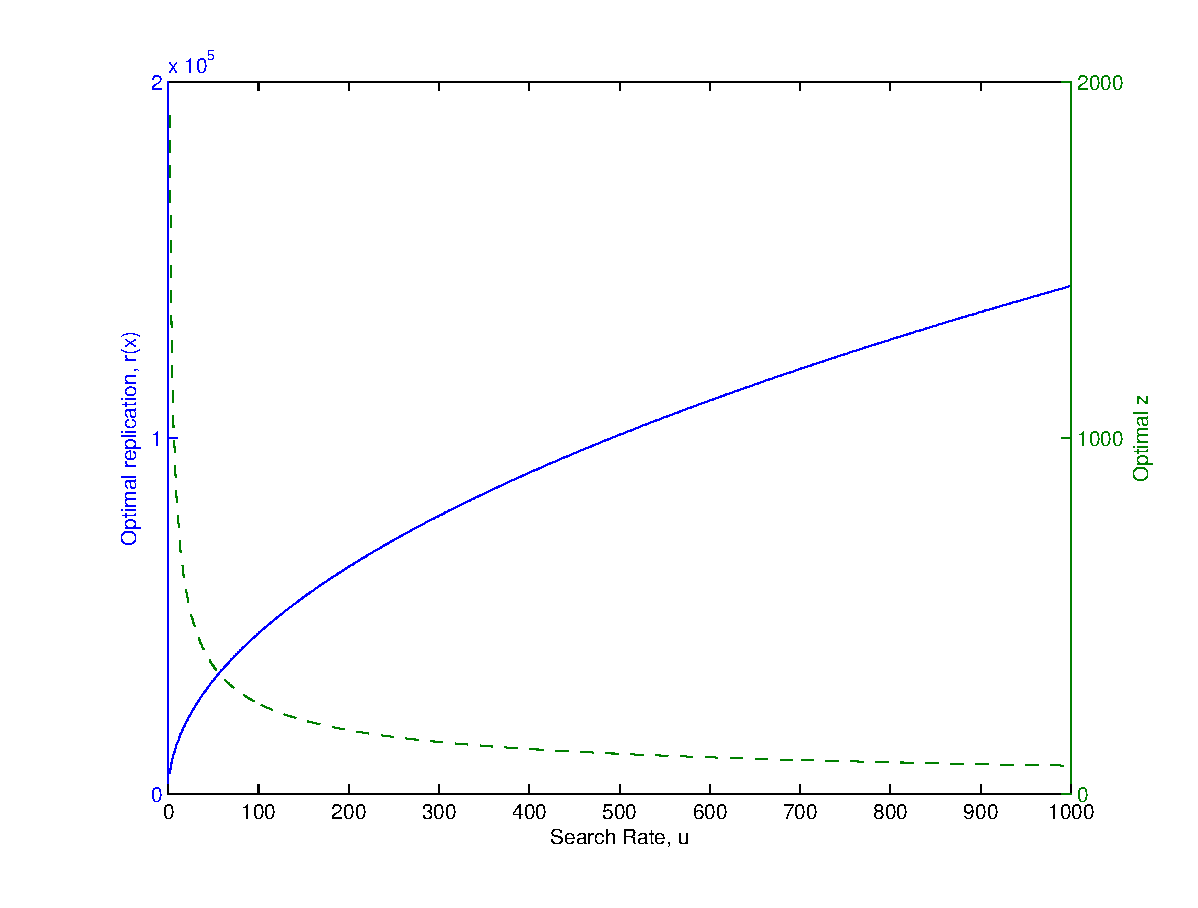
\includegraphics[width=0.5\textwidth]{Images/OptimalReplication.eps}
        \caption{The optimal bootstrap replication, $r(1)$, and $z$ values required to minimise the communication cost for a torrent with $u$ concurrent searches being performed for it.}
        \label{fig:optimal_replication}
    \end{figure}

    The authoring node of a torrent is unlikely to be aware of the torrent's popularity before releasing it. It is therefore difficult for the authoring node to determine the optimal starting replication, $r(1)$. It also difficult to know what value of $z$ is best suited for a torrent with an unknown popularity. Currently, our system will continue to increase the replication of a torrent's tracking data as the torrent gains popularity. A dynamic $z$ value could be used to ensure that the replication remains as close to optimal as possible. This is left as future work.

\subsection{Single Node Responding to Multiple Queries}

    In order for searches to be successful, queried nodes must respond to requests made of them. In order to estimate the communication cost of providing responses we need to know the number of times a node will be contacted and how large each response will be. When searching for a node, the expected number of requests made is $zP(d_i)^{-1}$. In \cite{guo_measurements_2005} the authors observe that the average BitTorrent node will perform $q=1.33$ searches every hour.  This is supported by Internet usage reports from Cisco\footnotemark. We can now estimate the number of requests generated by the entire network every hour:

    \begin{equation}
        qz\sum_{j=0}^{n}{P(d_{n_j})^{-1}}
    \end{equation}

    \footnotetext{Cisco's Visual Networking Index (VNI) puts the total peer-to-peer file sharing bandwidth consumption at 4,656 PB per month in 2011. Assuming that files downloaded over BitTorrent are, on average, 1GB in size. This tells us that $\displaystyle 4656\times10^{15}\times10^{-9}$ files are downloaded every month and that $\displaystyle 4656\times10^{6}\times(24\cdot7\cdot\frac{52}{12})^{-1}=6,395,604$ downloads complete every hour. Assuming bandwidth speeds and request rates are constant, we have that BitTorrent users request nearly 6.5 million torrents every hour. We observed ~5 million nodes and therefore conclude that each node generates $q=1.28$ requests per hour}

    Where $d_{n_j}$ is the document that node $j$ is searching for. These requests will be split uniformly over all of the nodes, each receiving an expected $\tfrac{1}{n\text{th}}$ of the total. To derive an estimate for the number of requests each node is likely to received every hour we can use the mean popularity of the torrents we observed in Section~\ref{sec:measurement}, 27. Table~\ref{tab:single_node_response_bandwidth} shows the expected number of requests received by a node per hour for different values of $z$ and $r(1)$. Each of the received requests requires a response, the size of the response depends on the node's awareness of the torrent requested. A node's awareness of torrents will increase the longer it remains in the network. Again, for simplicity, we shall assume that the node will always respond with the details of $a=1,10,\textrm{ or }100$ nodes. This simplification gives us the upper bound on the cost of responding, see Table~\ref{tab:single_node_response_bandwidth}:

    \begin{align}
                          R &= \textrm{requests recevied} \\
                            &= \frac{1}{n}qz\sum_{j=0}^{n}{(1-(1-\frac{r(27)}{n})^z)^{-1}} \\
                            &= \frac{qz}{1-(1-\frac{r(27)}{n})^z} \\
        \textrm{total cost} &= (68 + 6a)R
    \end{align}

    \begin{table}
        \renewcommand{\arraystretch}{1.3}
        \caption{The expected bandwidth (bytes/sec) used by a node for responding to queries.}
        \label{tab:single_node_response_bandwidth}
        \centering
        \begin{tabular}{l|l|l|l|l|l}
            \hline
            \multicolumn{2}{c|}{Strategy} &               ~ & \multicolumn{3}{|c}{Multi-request Response Cost (bytes/sec)} \\ \hline
              z &                     r(1) & \#requests/hour & $a=1$ & $a=10$ &                                      $a=100$ \\ \hline
            100 &                     1000 &             438 &     9 &     16 &                                           81 \\
            500 &                     1000 &             736 &    15 &     26 &                                          137 \\
            500 &                     5000 &             736 &    15 &     26 &                                          137 \\
           1000 &                     5000 &            1332 &    27 &     47 &                                          247 \\
            \hline
        \end{tabular}
    \end{table}

    In the worse case scenario ($z=1000$ and $r(1)=5000$), we observe that queried nodes would expend no more than 247 bytes/sec, an amount easily provided, given current home broadband capabilities.

\subsection{Global Bandwidth}

    The total traffic generated by a PAC Search system over BitTorrent can be estimated by taking the product of the number of requests generated by each node, the number of nodes and the average cost of a request and response. As in the previous section we use the popularity of the average torrent for simplicity:

    \begin{align}
        \frac{nqz(183 + \frac{6ar(27)}{n})}{1-(1-\frac{r(27)}{n})^z}
        \label{eq:overheads_global}
    \end{align}

    where $q=1.33$ is the query rate and $n=5,000,000$ is the number of nodes in the network. The expected global communication costs are given in Table~\ref{tab:global_bandwidth}. For low $z$ and $r(1)$ values we see a very small increase in global traffic, less than a quarter of 1\%. For larger values we see a much larger increase, just over 7\% in the worst cases. The cost of each strategy represents the expected costs incurred for successful searches, so we do not increase the failure rate by decreasing $z$ and $r(1)$. These data would suggest that low valued strategies are best if one wishes to reduce overall bandwidth consumption. These costs may be further reduced by applying a dynamic $z$ strategy, as discussed in previous sections.

    \begin{table}
        \renewcommand{\arraystretch}{1.3}
        \caption{Global bandwidth estimates in gigabytes per second for four different strategies of $z$ and $r(1)$ and three choices of $a$. The percentage increase over current global P2P traffic is also given.}
        \label{tab:global_bandwidth}
        \centering
        \begin{tabular}{l|l|l|l|l}
            \hline
            \multicolumn{2}{c|}{Strategy} &           \multicolumn{3}{|c}{Global Bandwidth Cost (GB/sec)} \\ \hline
            z &                       r(1) &         $a=1$ &        $a=10$ &      $a=100$  \\ \hline
          100 &                       1000 &   4 (+0.24\%) &   4 (+0.24\%) &   4 (+0.24\%) \\
          500 &                       1000 &  35 (+1.96\%) &  35 (+1.97\%) &  36 (+2.03\%) \\
          500 &                       5000 &  35 (+1.96\%) &  35 (+1.97\%) &  36 (+2.03\%) \\
         1000 &                       5000 & 126 (+7.09\%) & 126 (+7.11\%) & 130 (+7.32\%) \\
            \hline
        \end{tabular}
    \end{table}

\subsection{Storing the Index}

    In addition to using bandwidth to query and respond, each node must keep a local index of the torrents and nodes it is aware of. If we assume that each received request is for a distinct torrent then each item in the index will require 26 bytes, 20 for the infohash and 6 for the node's IP and port details. For a received-request rate, $s$ per hour, and total hours of operation, $h$, the local index size has an upper bound of $26sh$. The local index increases in size at a constant rate. In practise, requests will be received for torrents that are already in the index and so will only require an additional 6 bytes per request. Therefore we show here the worst-case scenario.

    Using the values in Table~\ref{tab:single_node_response_bandwidth} for the expected number of requests received per hour we can build an estimate for the upper bound of the local index.  The highest received-request rate in Table~\ref{tab:single_node_response_bandwidth} is 1332 per hour. At this rate a node's local index would reach 1GB after 28,876 hours, or 3.3 years of continuous use. For the lowest received-request rate we would see an index reach 1GB after 10 years.

    We see that the index size remains comfortably small even after extended usage. We consider then, that the most pressing reason for removing data from the index is to remove incorrect data. Data that suggests that a node owns a torrent when it does not. We offer three strategies for removing incorrect data:

    \begin{LaTeXdescription}
        \item[Least Recently Used] The local index is restricted to a small number of entries. When this entry limit is reached the oldest record is removed in order to make room for new ones. This method guarantees an upper bound to index size.. Unfortunately, it may remove perfectly good records from the index just because they happen to be the oldest. It may also do this when there exists incorrect data elsewhere in the index.
        \item[Periodic Ping] This is the method employed by the BitTorrent DHT to ensure that records are always relatively up to date. When a record is added to the index a timer is set up that regularly pings the node to check if it is still online. If it is not online then it is marked as potentially incorrect. If a node receives several ``incorrect'' marks in a row then it is removed. This method will rarely remove good data from the index and potentially bad data is marked as such. Unfortunately, it requires additional bandwidth as nodes have to be periodically pinged.
        \item[Timed] This method involves simply removing a record from the index when it has been there for a certain amount of time. As with least recently used, this method may remove good data.
    \end{LaTeXdescription}

    We imagine that a combination of either timed or least recently used with periodic ping will provide the best solution. When a record is considered for deletion, the node is pinged to check for correctness. If the record was in fact correct then it is left in the index. If the record is incorrect it is removed. We leave the analysis of these (and other) solutions as future work.